\section{Results}\label{sec:results}
In this section we report the results for our baseline and different configurations for finding utterance embeddings.
Also we present some analysis of our distributional representations.

\subsection{Baseline}
As a baseline we use a Bag-of-Words (BOW) representation.
We represent each utterance as a sparse vector, where every dimension maps to a word in the vocabulary.
We then train a Naive Bayes(NB) model and a K-Nearest Neighbor (KNN) classifier on the dialog act tagging task, both for the full tag set of 42 tags as well as on the aggregated tag set of eight tags.
Note that we could not train a Multilayer Perceptron (MLP) for the baseline due to memory constraints.
The results can be seen in Table~\ref{tab:results}. The strongest baseline we found was $59.98\%$ accuracy with the NB classifier.
Furthermore we calculated a trivial baseline where every utterance is classified as the most frequent dialog act tag, this would result in an accuracy of $31.47\%$.

To compare our results to those of the state of the art models proposed in earlier work we present their accuracy score in Table~\ref{tab:sota}. These models were evaluated on the same test set.
\begin{table}[t]
	\centering
	\begin{tabular}{r|r}
		& \textbf{accuracy} \\ \hline
		\newcite{kalchbrenner} & 73.9 \%           \\
		\newcite{stolcke2000}  & 71.0 \%           \\
		\newcite{milajevs}     & 63.9 \%          
	\end{tabular}
		\caption{Accuracy scores from other work}
		\label{tab:sota}
\end{table}

\subsection{Classification using Utterance Embeddings}
We inferred embeddings for utterances as discussed in section \ref{sec:utt2vec}.
Different setting were used to find these embeddings. We varied the training data, used 50 training epochs and pretrained word embeddings.
With these utterance embeddings we trained Naive Bayes (NB), K-Nearest Neighbors (KNN) and Multilayer Perceptron (MLP) classifiers.
In Table~\ref{tab:results} the results are presented.
As the results suggest, none of the methods could reach the BOW baseline set up by the Naive Classifier.
At least the high quality of the word embeddings is confirmed by the fact that the BOW baseline of the KNN method is outperformed by the utterance embeddings.

\begin{table*}[]
\centering
\begin{tabular}{r|lll|lll}
                   & \multicolumn{3}{c|}{\textbf{full tagset}} & \multicolumn{3}{c}{\textbf{aggregated tagset}} \\
                   & \textbf{NB}      & \textbf{KNN}     & \textbf{MLP}     & \textbf{NB}     & \textbf{KNN}     & \textbf{MLP}     \\
\hline
baseline BOW      & 59.98\%  & 39.57\% & -       & 72.71\%& 49.61\% &  -         \\
SWDA               & 38.18\%        & 54.55\%        &  50.32\%       &  59.55\%      &  70.82\%       &  66.76\%       \\
SWDA+BNC         & 38.16\%        &  53.86\%       &  51.40\%       &  60.10\%      &  68.75\%       &  68.39\%       \\
SWDA concat      & 27.24\%        & 33.29\%        &  51.42\%       & 51.21\%       &  43.87\%       &  67.98\%       \\
SWDA+BNC concat  & 25.02\%        & 34.07\%        &  51.68\%              & 51.68\%       & 44.64\%        & 68.36\%                \\
\end{tabular}
\caption{Tagging accuracies for different models and tagsets. All models were trained with 50 iterations and pretrained word embeddings.}
\label{tab:results}
\end{table*}


\subsection{Using context}
To use the contextual information of the dialog to classify dialog act tags, we experimented with two simple approaches. We either concatenated or summed the embedding of the previous utterance to the embedding of the current one.
The first approach nicely represents the sequentiality of the dialog but it doubles the amount of features for the classifier to consider.
The latter approach is not affected by this curse of dimensionality, however it does lose all sequential information present in the dialog.
As expected, the latter approach would not yield any improvement. On the contrary, the tagging accuracies are worse when utterance embeddings are simply added.
For that reason we did not follow that approach any further.
The results for the concatenation of utterances (concat) can also be seen in Table~\ref{tab:results}.

\subsection{Error Analysis}
Utterance embeddings have the property of encapsulating the meaning of utterances from the words that compose them; as with the case of word embeddings, these representations present appealing relations from which similar words (in a semantic sense) appear close by in the high dimension space.
We extract samples from the SWDA corpus belonging to tags that are clearly unrelated and apply dimensionality reduction to their vector representations using Principal Component Analysis (PCA).
We plot the results in three dimensions.
The sampled utterances belong to the following categories: \emph{Wh-question}, \emph{Thanking}, \emph{Reject}, and \emph{Apology}.
Considering the words that are used in these kind of units, sample points should be clearly separated.
The utterance embeddings were extracted using a 300-dimensional model trained on the SWDA corpus using pretrained word vectors.
Figure~\ref{fig:4cat_3d_pca} shows the utterance embeddings in 3D after applying PCA.

\begin{figure}
\centering
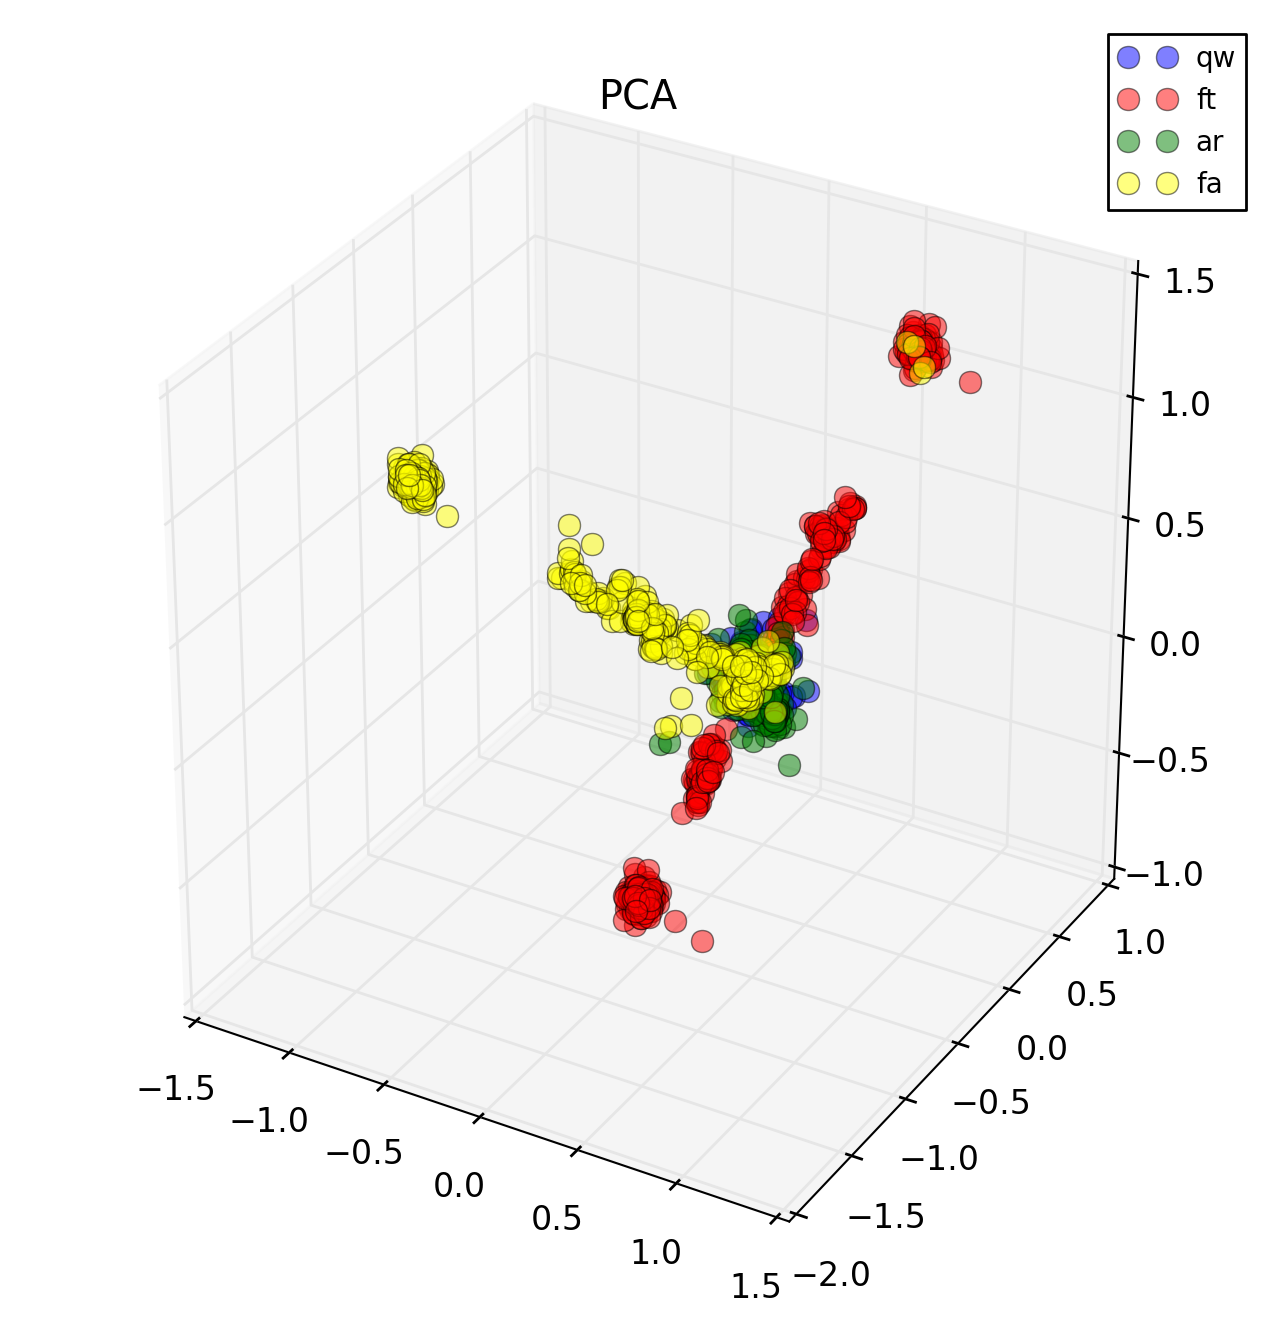
\includegraphics[width=\columnwidth]{img/easy_pca_3d}
\caption{3D PCA.}
\label{fig:4cat_3d_pca}
\end{figure}

Though, the classification task seems easy considering the previous tag examples, it gets more complicated when we handle other types of utterances.
Figure~\ref{fig:5cat_3d_pca} shows the diagram after applying PCA to utterance embeddings of the five most frequent tags (\emph{Statement-non-opinion}, \emph{Acknowledge}, \emph{Statement-opinion}, \emph{Accept}, \emph{Turn exit}), which account for $78\%$ of the corpus.

\begin{figure}
\centering
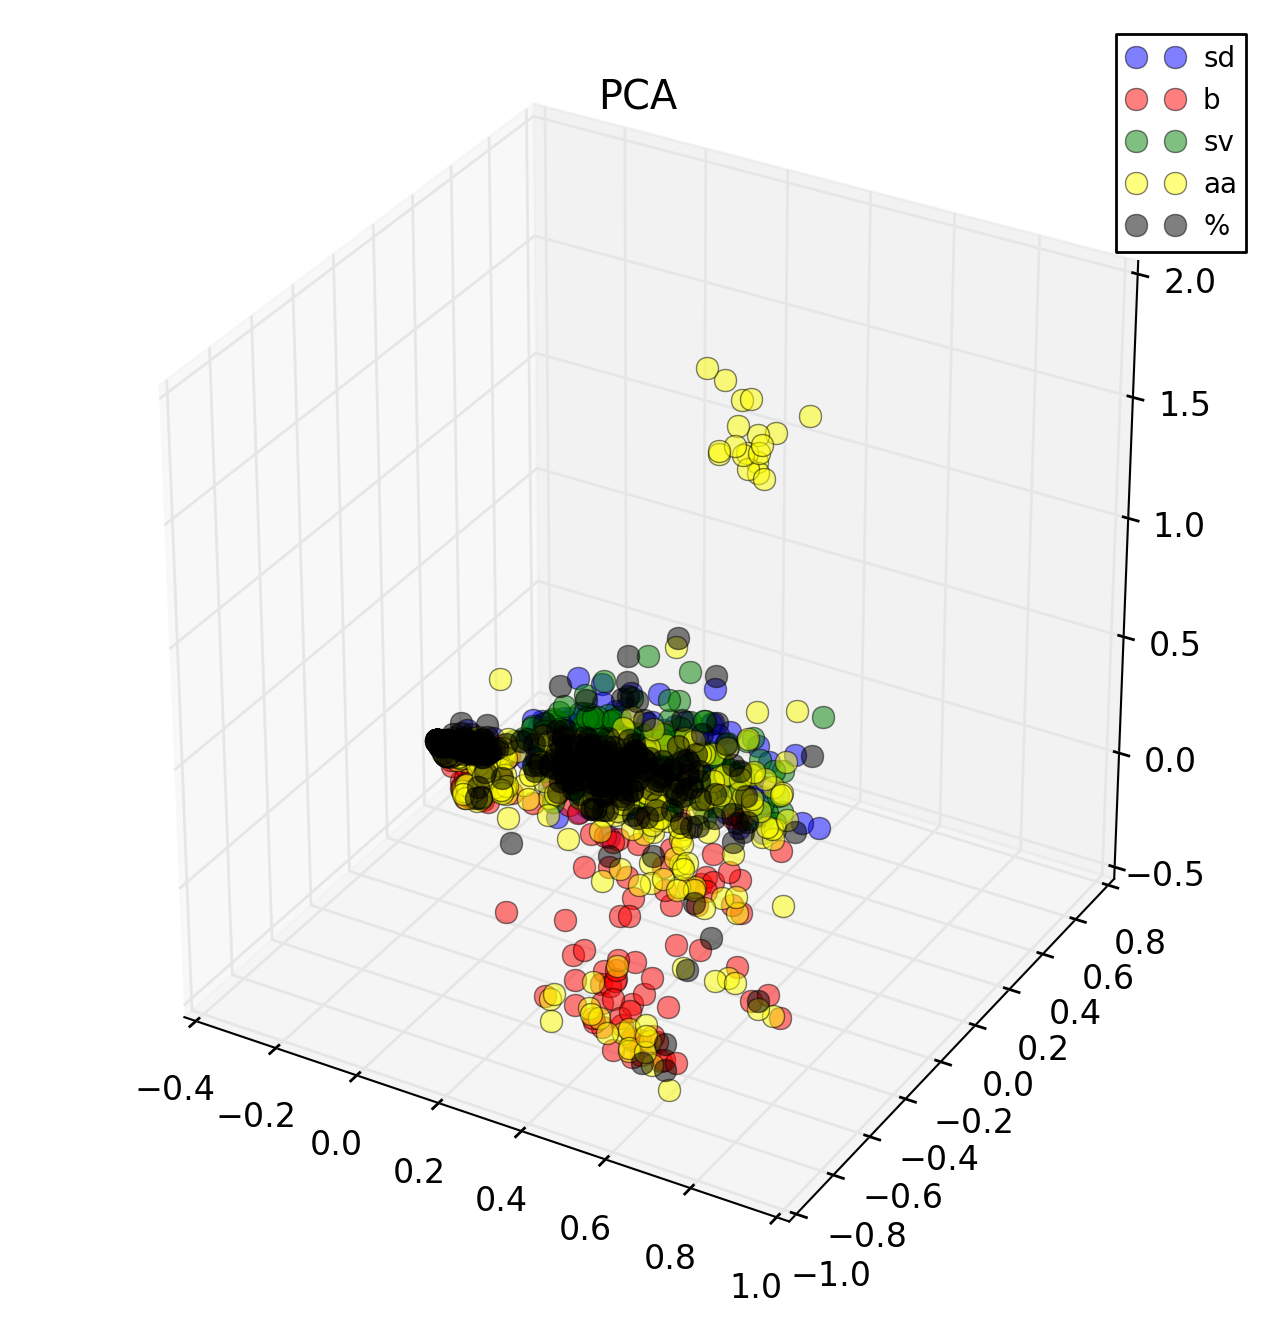
\includegraphics[width=\columnwidth]{img/complex_pca_3d}
\caption{3D PCA.}
\label{fig:5cat_3d_pca}
\end{figure}
